\chapter{Related work}
\label{ch:related_work}


This chapter reviews approaches made towards handling Known-item Search (KIS) task and the recent approaches for user-friendly traverse through the immersive amount of the visual data.

In recent years, we witnessed a significant advancement in the solution for the KIS task. The scale of the solution's complexity for user interaction ranges from simple ones (e.g., sketching color blocks) with only a few descriptors to the ones which use recent advance in deep learning, as for concept labeling (i.e, naming objects).

Our goal is to perform known-item-search task on a set of videos. We perform a common simplification, replacing videos with the set of images. We do this, since we look for a particular scene, which can be also an image. This level of abstraction therefore corresponds to the searched query. Also, this allows us to use a potential of a common neural networks and other solutions presented for 2D data (images in our case). For this task we perform sampling over the videos. More information is available in section \ref{}\todo{fix}, where more details about the dataset are available.

\section*{Known-item-search Task}

Known-item-search task is present in many different situations. The tasks is to efficiently retrieve a known item in the dataset. For example, for a database of newspaper article we may use such retrieval tools to find a particular article we are interested in. Our thesis focuses on visual KIS task, specifically we retrieve images. For the setting we solve our task in exist even annual competitions to share the knowledge and the advancements. One of such is Video Browser Showdown \ref{}\todo{fix}, which is taking place since 2012. We review a few of the presented solutions to this task from the last VBS2019. We mainly follow the summarization in the \ref{}\todo{fix}

The most common approach at the VBS2019 were "Query by an Image" and "Concept Labeling". Query by an image, in this case, mostly refers to finding the most similar results from databse to given image. The downside of this approach is mainly the difficulty to obtain an image, which would be sufficiently similar to the searched one.

The second most used approach at VBS2019 was Concept Labelling. In this case, a user can describe the scene using the words. The database is pre-annotated with the vocabulary of present items. During the request, the algorithm checks the database for the presence of the searched concept. This approach has a limitation of the vocabulary size. Recent advancement in the textual annotation neural networks is nowadays able to describe thousands of different objects by words, but still, this may present on the limitation on rarely used objects or hard to describe objects.

One of the approaches presented and used is by creating a color sketch. The user colors the canvas with respect to the original searched scene. The database is then traversed on the correspondence of the colors to the particular part of the image. We see a significant advantage of this approach to distinguish between the key objects in the scene spatially.
 
Solving KIS task in VBS setting offers the option of using full video information and not only snapshots. This approach enhances the possibilities spectrum to Temporal Queries or Multimodal queries. Also, the solution included Optical Character Recognition (OCR) was presented. We present our solution as a possible enhancement of a complex system in order to create multiple search strategies based on user-preference. 

\section*{Traversion Approaches}

Since the KIS task is the task of two sides -- the algorithm and the user, it is essential to not forget about the easy to use interface. A good overview of the dataset may hide some deficiencies of the algorithm so that the user can still find the search scene. As the  (Evaluation of VBS ref)\todo{fix} shows, the most common approach is to show a 2D grid of images to the user. Several approaches also provide an easy way to play the original video as one of the most immersive ways we have encountered to traverse a grid of images is placing these images on the globe with the possibility of multiway traversing (TODO: ref). We aim to achieve a similar level of smooth traversing.

The traversing systems rely on effective visualization techniques on high-number feature spaces. These systems create mostly a 2D grid of the images based on the distance between the samples in high dimensionality space. Though, this high dimensionality space, often produced by neural networks, may not have feasible representation in 2D space based on the hidden features. This is often caused by a lack of understanding and representability of the deep features. We aim to test this feature reduction to the 2D test in our face experiment with the use of deep neural network features.

\section{Existing systems}

In the next section we shortly investigate on existing frameworks, which competed in the Video Browser Showdown.

\subsection{VIRET}

A framework named VIRET (\cite{lokovc2019framework, lokovc2019viret}) is successfully participating in the competitions for a several years now. The framework evolved in the years and now it offers a wide variety of the strategies for solving KIS task. VIRET also implements own strategy for a frame selection, which we also used for obtaining our images. As one of the biggest strategical advantages of the VIRET we consider a multi-modal queries with relevance scores and update of the queries based on the results. We take VIRET as our inspiration and we do not implement the same approaches as are already present in the VIRET. We focus on testing new alternatives.

\begin{figure}
    \centering
    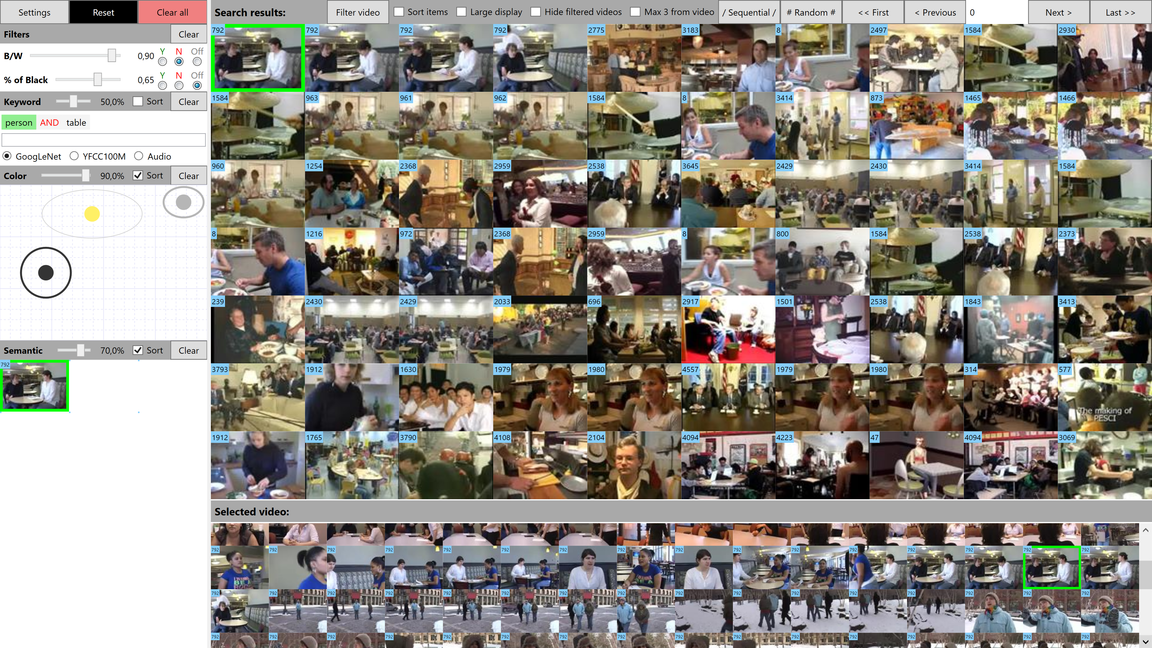
\includegraphics{img/viret_small.png}
    \caption{A sample search in VIRET framework. Source: https://videobrowsershowdown.org/hall-of-fame/}
    \label{fig:viret}
\end{figure}

\subsection{SOM Hunter}

A SOM Hunter (\cite{kratochvil2020som}) was for the first time introduced at the VBS2020. This tool is related to us, since it successfully proved using Self-organizing Maps for a use in a Known-item-search task. They train a small self-organizing map on the fly over only a sample of the dataset. This allows them to recreate the SOM based on the user interaction and train it on the fly. In our work we use the idea of training SOM, but compared to the SOM Hunter we will test creating a SOM only on the faces of the people.

\begin{figure}
    \centering
    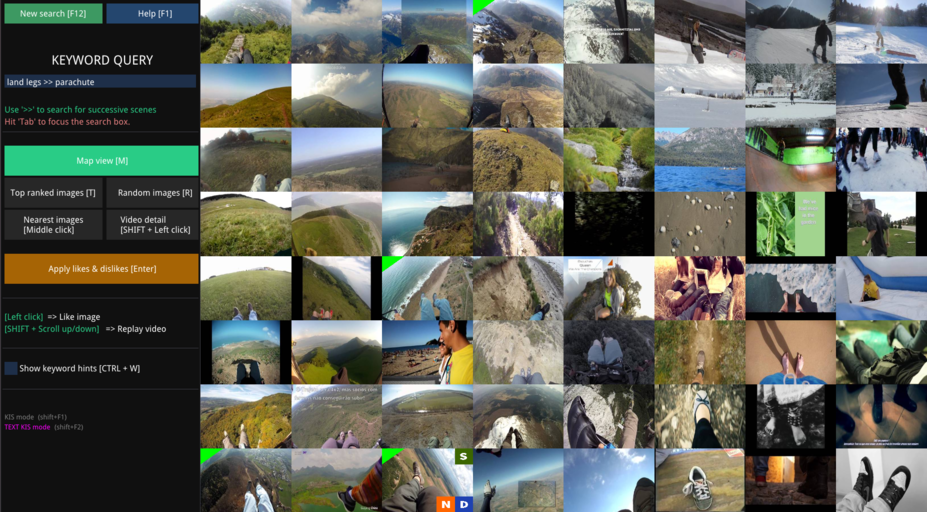
\includegraphics[width=0.99\linewidth]{img/som_hunter_small.png}
    \caption{A sample search in SOM Hunter. Source: https://videobrowsershowdown.org/hall-of-fame/}
    \label{fig:som_hunter}
\end{figure}

\subsection{Vitrivr}

Vitrivr (\cite{rossetto2016vitrivr}) is one part of more complex solution for retrieving a video in the collection. Vitrivr is the module responsive for creating queries which are then processed by the Cineast. The overview of the system is displayed in the figure \ref{fig:vitrivr}. The Vitrivr supports different query types, as query by a sketch, example image, semantic concept, keywords, audio or motion. The feature extraction and the system behind retriving the most similar results are part of the second module -- Cineast (\cite{rossetto2016searching}). Cineast uses multiple approaches incorporating deep features, i.e. scene text recognition and speech-to-text recognition. The Vitrivr (part responsible for creating the queries) is a web-browser solution, therefore the tool includes a clean separation between the query formulation and retrieving the responses.

\begin{figure}
    \centering
    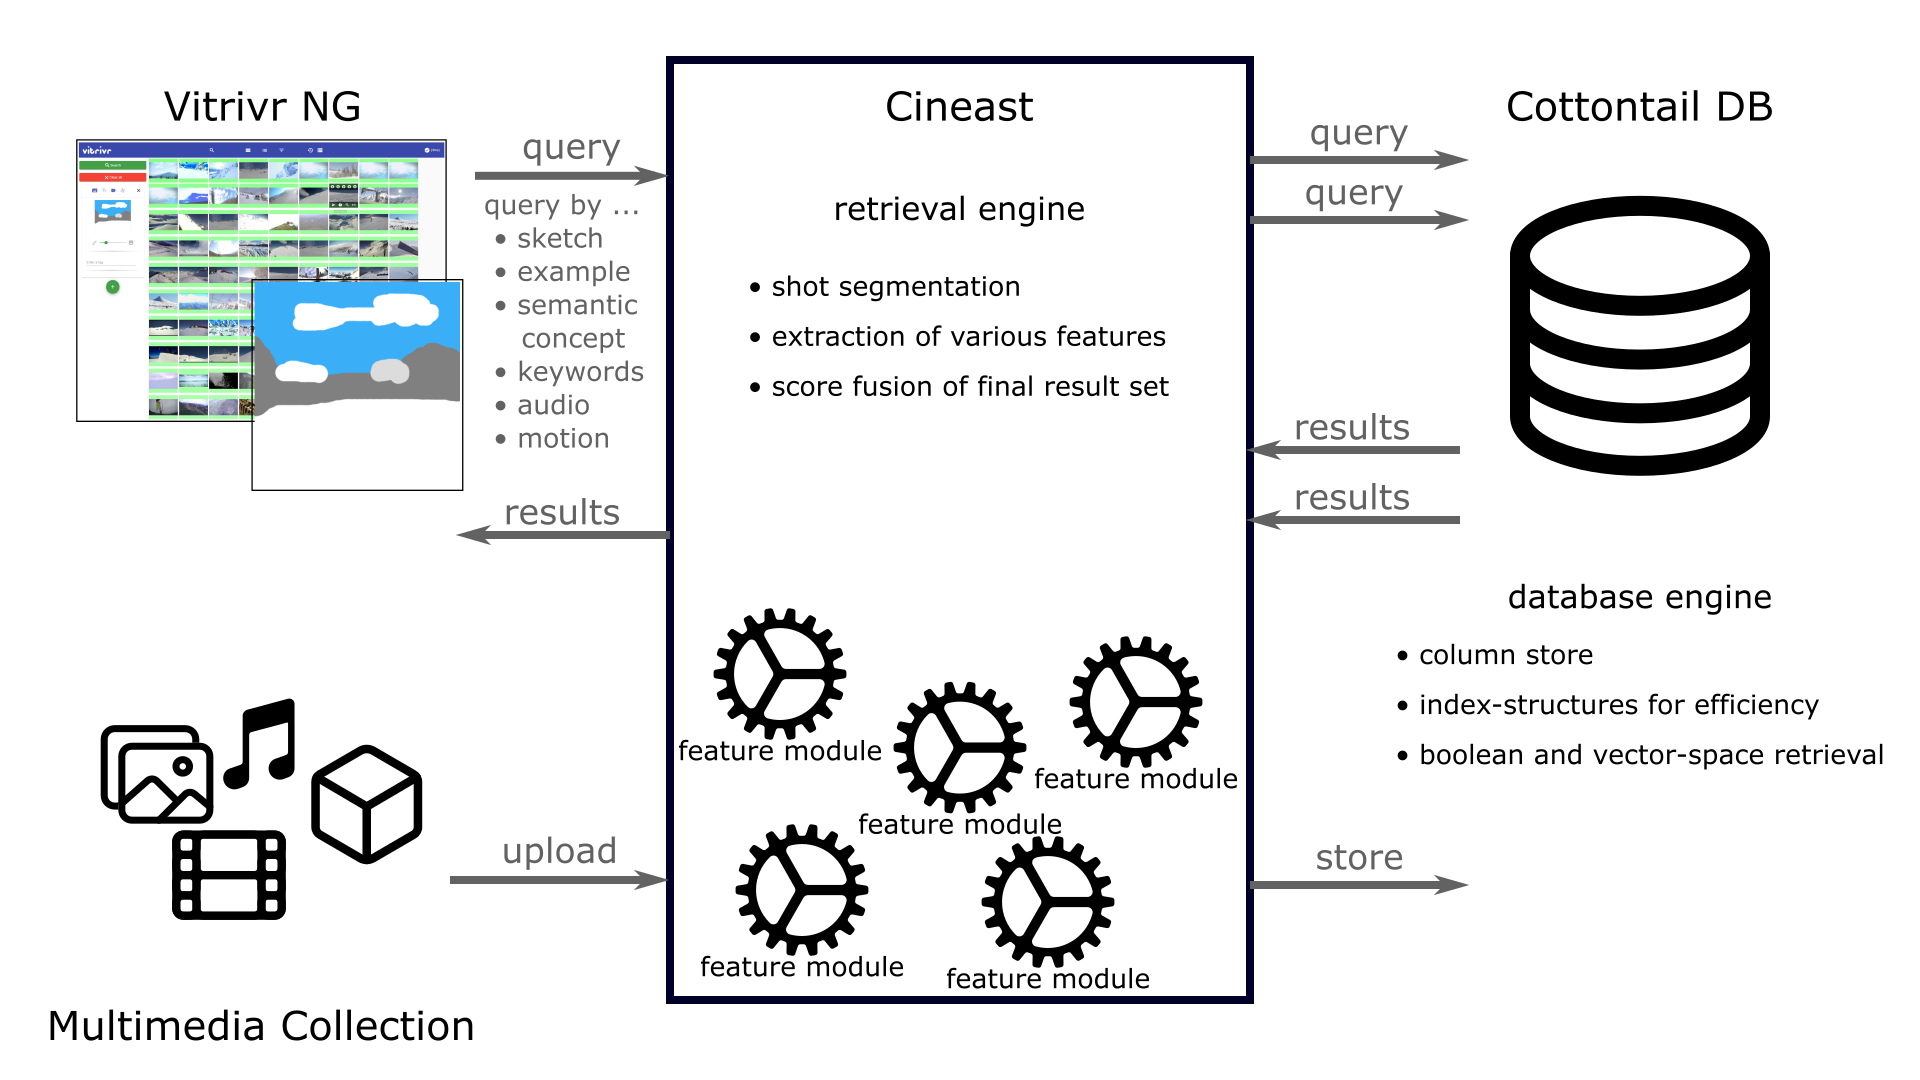
\includegraphics[width=\linewidth]{img/vitrivr.png}
    \caption{Overview of the separation in the Vitrivr solution. Source: \url{https://vitrivr.org/vitrivr.html}}
    \label{fig:vitrivr}
\end{figure}

\section{Deep Neural Networks}

In recent years we witnessed many records-breaking new machine learning models. Many of those were possible, thanks to the advancement of Deep Neural Networks (DNN). Nowadays, these models replaced more traditional Machine Learning approaches in many tasks.

Deep Neural Network is a machine learning model, whose goal is to approximate a given function \(f\). The set of parameters is often referred to as \(\theta\). One of the everyday tasks performed by these networks is classification, where the goal of the network is to predict which category sample \(X\) belongs. Even though we will not perform a classification task in this thesis, we will use some of the available classification networks.

When we talk about neural networks, we usually refer to a feedforward network. These networks consist of layers where information during the evaluation is passed only in one direction. We can imagine it as applying a function to the results from the previous layer. For example, let us create a small neural network. Denote first layer as \(f_1\) and second layer as \(f_2\). The output of the network will be \(f_2\left(f_1\left(\right)\right)\).

Stacking more and more layers on top of each other leads us to notation \emph{deep} neural networks. This notation has no fixed threshold on which networks "deserve" to be called deep. Therefore we do not recognize any importance to the naming "deep." 

The first and last layer are commonly referenced as \emph{input} and \emph{output} layer. Layers between the input and output layers are usually denoted as \emph{hidden} layers. Deep neural networks can have four or hundreds of layers, and each layer of the layer can have even a unique structure. \emph{Network Architecture} captures the "build order" of the network. It is important to note that there exist many networks with different architectures solving the same task.

There are many reasons for the advancement of neural networks in the past years. One of the crucial stones was not only theoretical innovations used for the networks but increasing computability limits. Deep Neural Networks \emph{learn} to approximate function by \emph{training}. This training is usually the heaviest part of the computation. Even though it is enough to train once and use forever, it usually lays some limitations on the size of the networks or the functions used.

Since this topic is broad, we recommend more thorough reading, such as Neural Networks and Deep learning online book\footnote{http://neuralnetworksanddeeplearning.com/}.

\subsection{Convolution Neural Networks}

Convolution Neural Networks (CNN) are a class of Deep Neural Networks. Even though they emerged in the late 1980s (\cite{lecun1989backpropagation}), it took another 20 years for further advancements in the research area. Convolution Neural Networks are mainly used in image-related tasks, such as image classification ("What is on the image?"), object detection ("Where are the objects in the image and what are they?") or even content generation ("Create a new image"). Their abilities were also tested in many, not image-related tasks, e.g., music genre recognition.

Convolution Neural Networks are specialized kind of networks which work with grid-like topology. For 1D can be an example as time-series, or for 2D, most typically image pixels represent a grid. The name \emph{convolution} refers to using a mathematical linear function \emph{convolution} in at least the layers. A simplified overview of the structure is displayed in figure \ref{fig:convolution_neural_network}. We refer to \cite{Goodfellow-et-al-2016} for more understanding of \emph{convolutional layers}.

\begin{figure}
    \centering
    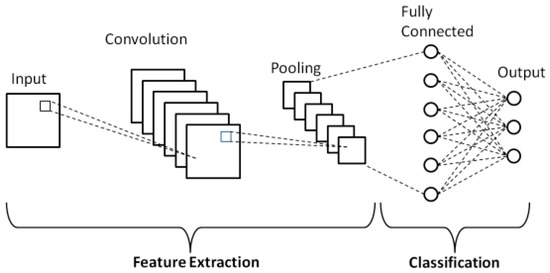
\includegraphics[width=0.98\textwidth]{img/convolution_neural_network.jpg}
    \caption{Schematic diagram of a basic convolution neural networks. Source: Phung, V.H.; Rhee, E.J. A High-Accuracy Model Average Ensemble of Convolutional Neural Networks for Classification of Cloud Image Patches on Small Datasets. Appl. Sci. 2019, 9, 4500.}
    \label{fig:convolution_neural_network}
\end{figure}

\subsection{Transfer Learning}

Transfer Learning is a research problem in machine learning that focuses on storing knowledge gained while solving one problem and applying it to a different problem. We have seen many successful transfers of the network architecture and parameters learned to a new task. Transfer learning helps to reduce the cost of the training and often also to overcome an insufficient set of training examples for the new task.

We utilize some of the pre-trained Convolution Neural Networks. The ability of a convolutional neural network to transfer to a new task by elevating gained information from other datasets was explored as early as by \cite{donahuedeep}, and many others were able to use this information to gain better models.  Networks we use are mostly pre-trained on \emph{ImageNet}\footnote{http://www.image-net.org/}. ImageNet served as a benchmark for comparing the performance of the different networks. Since the ImageNet is the main classification task, we utilize the transfer learning in a way to obtain deep features. Layers to the end of the networks accumulate more information, i.e., they contain high-level features. Therefore, we work with the layers close to the end of the networks. These layers represent encoded information about the image in high dimensional vectors. Our task is to use these deep features obtained for solving our known-search item task.


\begin{figure}
    \centering
	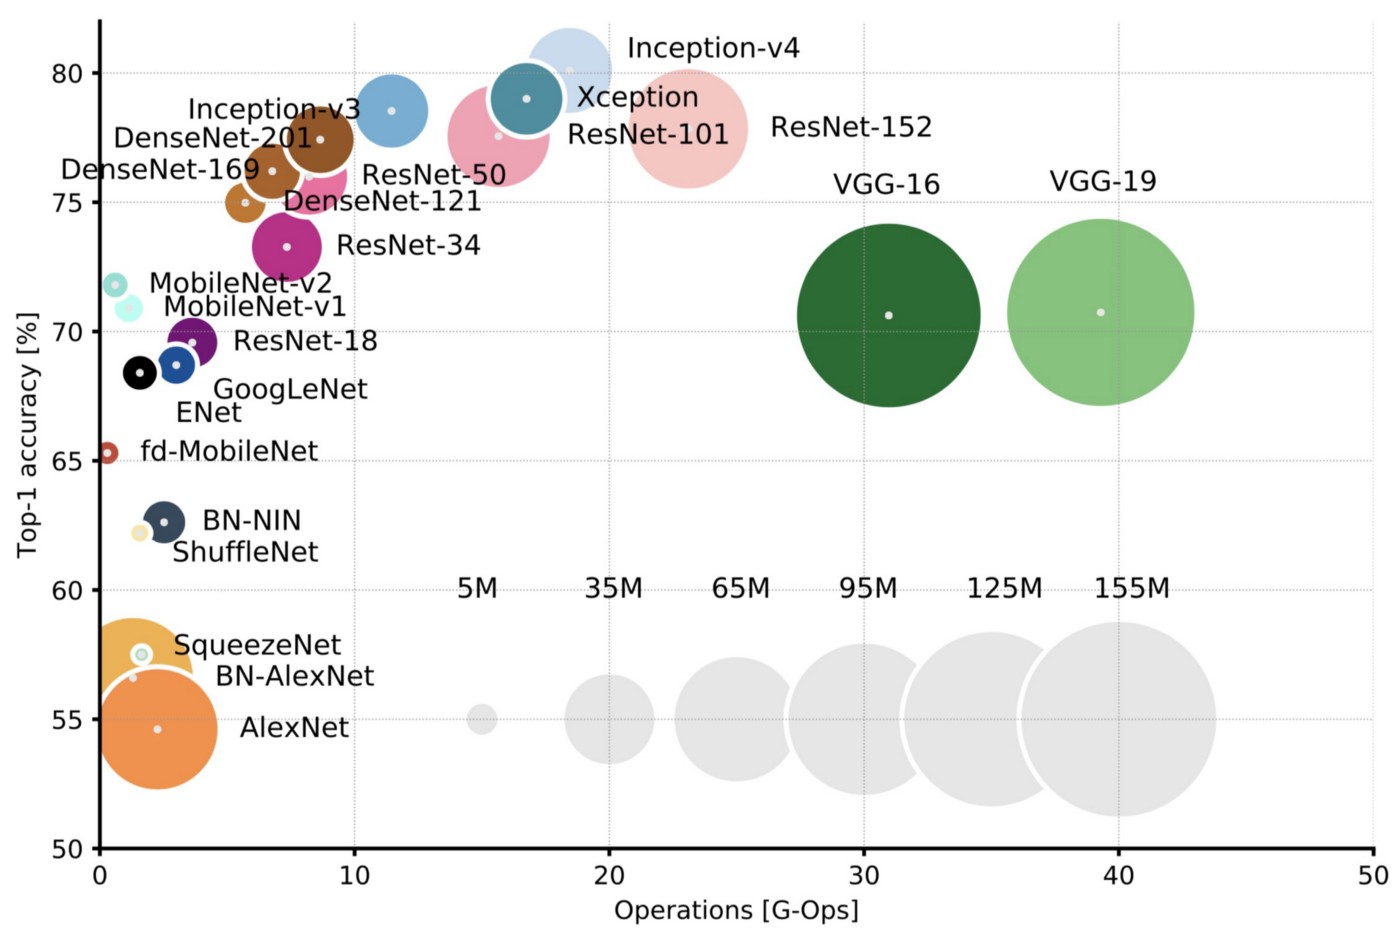
\includegraphics[width=0.8\linewidth]{img/network-comparison.jpeg}
	\caption{Top-1 one-crop accuracy versus amount of operations required for a single forward pass. The size of the blobs is proportional to the number of network parameters. Source: \cite{canziani2016analysis}}
	\label{fig:camera-setup}
\end{figure}

\subsection{Pretrained models}
\label{ss:pretrained_models}

\subsubsection{Keras}

Keras (\cite{chollet2015keras}) is a deep learning API written in Python, running on top of the machine learning platform TensorFlow\cite{tensorflow2015-whitepaper}. It was developed with a focus on experimentation in deep learning. We use it and its pre-trained models in this thesis. The models available in Keras Applications, which we use, were trained on ImageNet. Keras API allows us to separate the model from the last fully connected layer used for classification (since default ImageNet is a classification task). 

\subsection{Models Used}

\subsubsection*{Resnet50V2}
\cite{resnetv2} \cite{resnet}

\subsubsection*{MobileNetV2}
\cite{mobilenet} \cite{mobilenetv2}

\subsubsection{Dlib}
Dlib (\cite{king2009dlib}) is a modern C++ toolkit containing machine learning algorithms and tools for creating complex software in C++ to solve real-world problems. Some of the modules are provided with Python API. We use the Dlib library for face detection and also face feature extraction. For both we use face\_recognition API (\cite{geitgey2016machine}). \cite{king2017high} \todo{fix ref}




